%----------------------------------------------------------------------------
\label{doppler section}
%----------------------------------------------------------------------------
Consider the same two level system studied in section \ref{basic_two_level}. If we start with the same assumptions except instead of perfect resonance we allow for a small mismatch between the excitation field and the transition under consideration (i.e. $\nu\sim\omega_1-\omega_2$) we get
%----------------------------------------------------------------------------
\begin{subequations}
\begin{eqnarray}
\dot{c_0}
&=&
-\Delta
e^{i \xi \tau (\delta \omega)}
c_1
\\
\dot{c_1}
&=&
+\Delta
e^{i \xi \tau (-\delta \omega)}
c_0
\end{eqnarray}
\label{doppler eom}
\end{subequations}
%----------------------------------------------------------------------------
where $\delta \omega = \nu\ - (\omega_1-\omega_2)$, $\Delta\equiv\Delta_{10}=\Delta_{01}$, and $\ket{0},\ket{1}\in\{\ket{x}\}$. Of the two selectively coupled states, state $\ket{0}$ is the ``ground'', i.e. initially occupied; and state $\ket{1}$ is the targeted excited state, initially unoccupied.

The solution to \ref{doppler eom} is
%----------------------------------------------------------------------------
\begin{subequations}
\begin{eqnarray}
c_0
&=&
\exp{\left(
i \frac{\Phi}{2} \tau
\right)}
\left(
\cos{\left(
\frac{\Omega}{2} \tau
\right)}
-
i\sin{\left(
\frac{\Omega}{2} \tau
\right)}
\right)
\\
c_1
&=&
\frac{2 \Delta}{\Omega}
\exp{\left(
-i \frac{\Phi}{2} \tau
\right)}
\sin{\left(
\frac{\Omega}{2} \tau
\right)}
\end{eqnarray}
\end{subequations}
%----------------------------------------------------------------------------
where $\Phi \equiv \xi \cdot\delta\omega$ (dimensionless detuning) and $\Omega\equiv \sqrt{\Phi^2 +4\Delta^2}$. Now
%----------------------------------------------------------------------------
\begin{equation}
P_1(\tau)
=
\left( \frac{2 \Delta}{\Omega} \right)^2
\sin^2{\left(
\frac{\Omega}{2} \tau
\right)}
\end{equation}
%----------------------------------------------------------------------------
or
%----------------------------------------------------------------------------
\begin{equation}
P_1(\tau,\Phi)
=
\frac
{1}
{
1+\left(\frac{\Phi}{2\Delta}\right)^2
}
\sin^2{\left(
\Delta \tau \sqrt{1+\left(\frac{\Phi}{2\Delta}\right)^2}
\right)}
\end{equation}
%----------------------------------------------------------------------------
where $P_1(\tau)\equiv|c_1|^2$. This can be rewritten as
%----------------------------------------------------------------------------
\begin{equation}
\boxed{
P_1(t,\delta\omega)
=
\frac
{1}
{
1+\left(\frac{\delta\omega}{\Omega_R}\right)^2
}
\sin^2{\left( 
\frac{\Omega_R}{2} t \sqrt{1+\left(\frac{\delta\omega}{\Omega_R}\right)^2}
\right)}.
\label{final eom}
}
\end{equation}
%----------------------------------------------------------------------------

%----------------------------------------------------------------------------
%----------------------------------------------------------------------------
%bb defines the bounding box for the pdf
%viewport defines the area of the pdf used
%in sidewaysfigure the last entry in bb moves the caption toward/away the pic
%in sidewaysfigure the second entry in bb moves the pic toward/away the caption
%----------------------------------------------------------------------------
\begin{figure}
\scalebox{0.8}[0.8]{
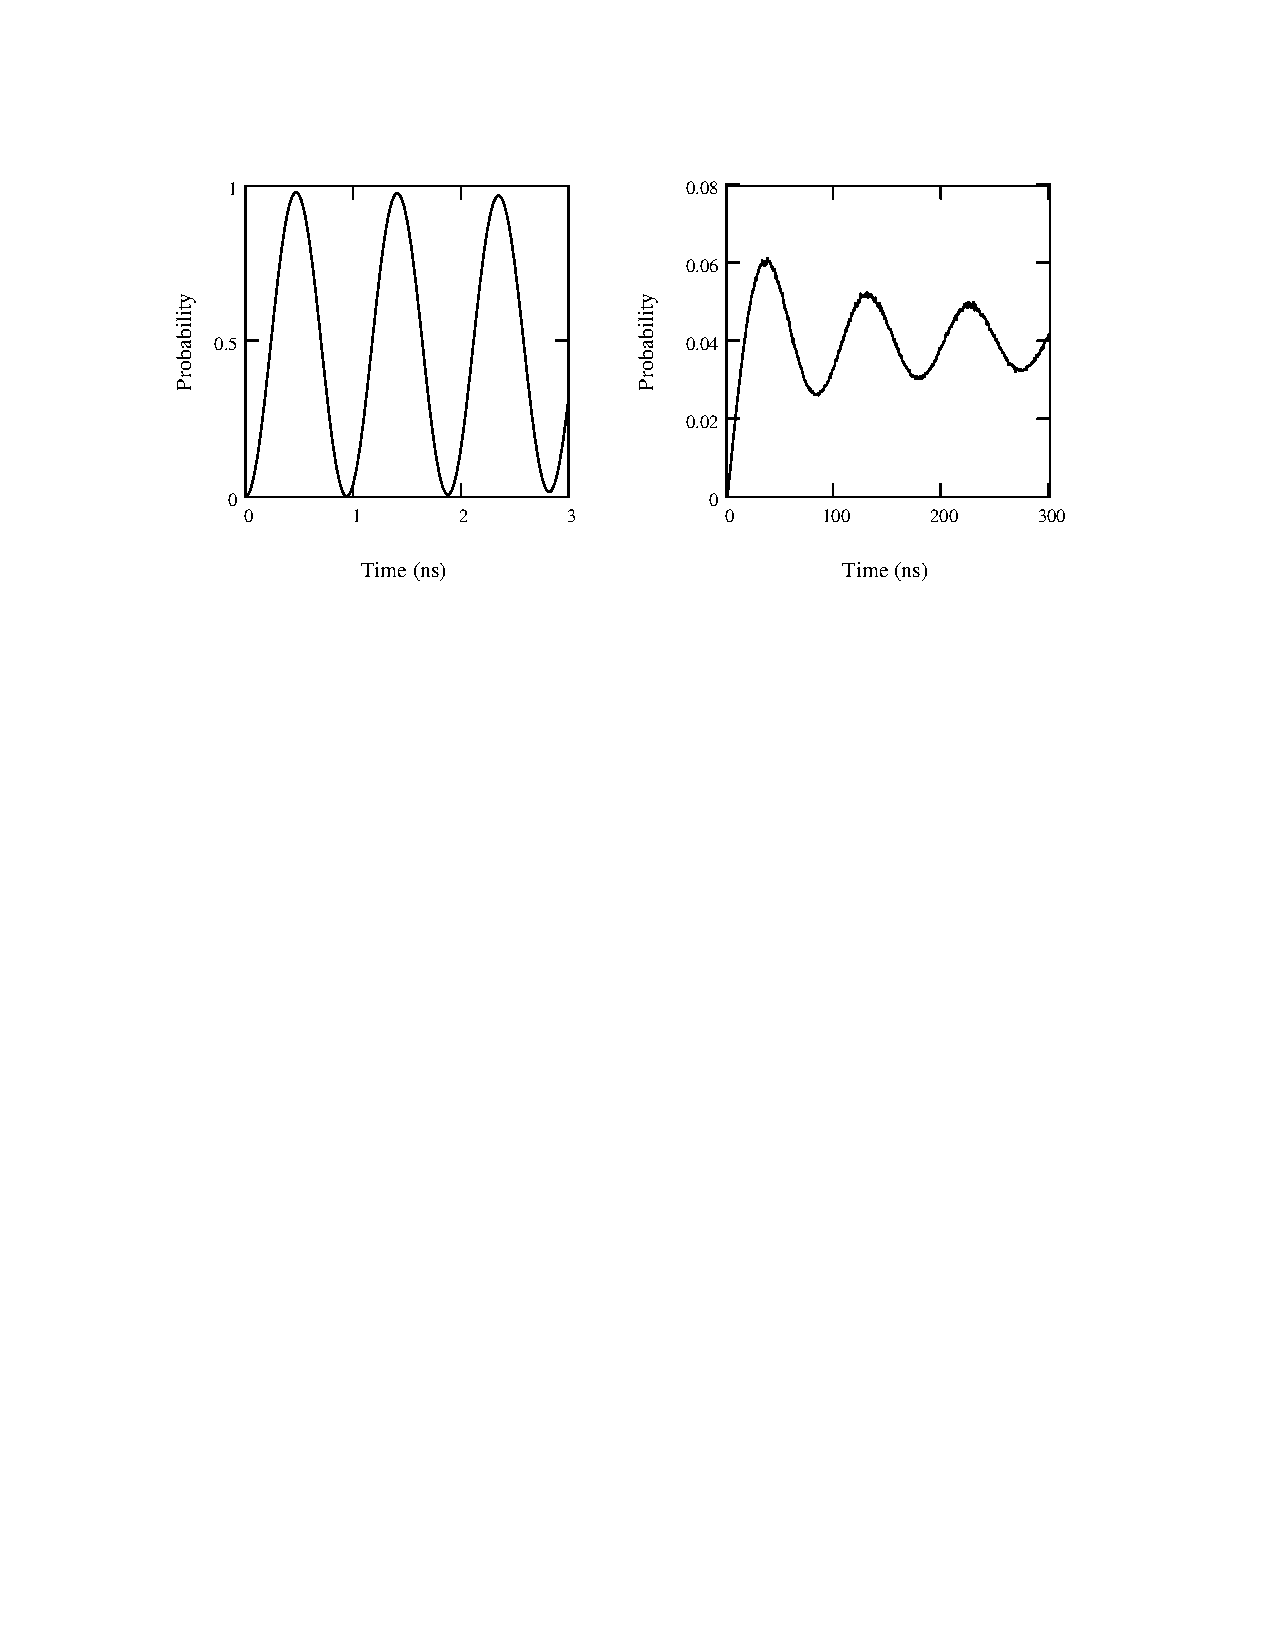
\includegraphics[bb=35 515 550 700]
{doppler_only/doppler_only.pdf}
}
\caption[Simulated thermal (Doppler only) effects on observed fluorescence -- high fluence vs. low fluence]{Simulated thermal (Doppler only) effects on observed fluorescence -- high fluence vs. low fluence. For these two simulations we use a fluence of 1000 J/m$^2$ for the left plot and a fluence of 10 J/m$^2$ for the right plot. The target is thermal molecular iodine gas with dipole matrix element $3.6\cross10^{-32}$ Cm (including FCF), at T = 293 K.}
\label{doppler_only}
\end{figure}
%----------------------------------------------------------------------------

%----------------------------------------------------------------------------
Clearly we would like to work in the limit $\delta\omega/\Omega_R<<1$ (this is equivalent to $\Phi/2\Delta<<1$); unfortunately, this ratio is near unity for ambient atmospheric targets excited with ns laser pulses. $\Omega_R$ must be faster than the relaxation processes in the atmosphere, about 1ns; thus $\Omega_R\sim$1 GHz. $\Delta\omega$ is forced to be at least 0.36 GHz due to Doppler broadening; however, laser line broadening produces an equivalent effect, thus the transform limit of the 1  ns laser pulse will place a lower limit on $\delta\omega$: again about 1 GHz. See Figure \ref{doppler_only} for a comparison between ``fast'' population transfer (using a 2 ns pulse) and a ``slow'' transfer (using a 200 ns pulse).
%----------------------------------------------------------------------------
%----------------------------------------------------------------------------
%----------------------------------------------------------------------------
